\documentclass[12pt]{article}
\usepackage{amsmath} %\mathcal
\usepackage{amssymb} %\mathbb
\usepackage{amsthm}
\usepackage{amsfonts}
\usepackage{graphicx}
\usepackage[utf8]{inputenc}
\usepackage{xcolor}

\newcommand{\sca}[2]{\left \langle #1 \middle| #2 \right \rangle} % inner product
\newcommand{\norm}[1]{\left\lVert #1 \right\rVert}
\newcommand{\RR}{\mathbb{R}} % espace réel
\newcommand{\CC}{\mathbb{C}} % espace complexe
\newcommand{\PP}{\mathbb{P}} % mesure de probabilité P
\newcommand{\QQ}{\mathbb{Q}} % mesure de probabilité Q
\newcommand{\EE}{\mathbb{E}} % espérance E
\newcommand{\ZZ}{\mathbb{Z}} % mesure de probabilité Z
\newcommand{\NN}{\mathbb{N}} % entiers positifs
\newcommand{\n}{\mathcal{N}} % Normal distribution
\newcommand{\Ss}{\mathcal{S}} % hyperspherical structure

\newcommand{\blue}[1]{\textcolor{blue}{#1}}
\newcommand{\red}[1]{\textcolor{red}{#1}}

\title{Notes on the article : Hyperspherical Variational Auto-Encoders}
\author{}
\begin{document}

\maketitle

\section{Expected project outcomes}
No report, only a 7-minute presentation :
un \textbf{très court résumé de la contribution proposée dans l'article} et surtout vous concentrer sur une \textbf{critique en lien avec le cours}.
Si c'est un article théorique, qu'apporte-t-il de plus que ce qu'on a vu en cours et est-ce un apport ou paie-t-on le prix ailleurs avec d'autres conditions ? \textbf{La preuve a-t-elle un schéma classique ?} etc..
Si l'article est méthodologique, \textbf{qu'en pensez-vous ? Pouvez-vous reproduire facilement les résultats de l'article avec votre implémentation ?}

\section{Contribution}
The Gaussian distribution is widely used in Variational Autoender models but it fails to model data with a latent hyperspherical structure. The authors replace it with the Von Mises-Fisher (vMF) distribution leading to a hyperspherical latent space.
Their experiments show that :
\begin{itemize}
    \item hyperspherical VAE, or $\mathcal{S}$-VAE, is more suitable to capture data with a hyperspherical latent structure,
    \item while outperforming a normal, $\mathcal{N}-VAE$, in low dimensions on other data types.
\end{itemize}

Some data types are better explained through spherical reprensentations like \textit{directional data}?? (e. g. protein structure, observed wind directions). Few machine learning techniques explicitly account for the intrinsically spherical structure of some data in the modeling process.
Uniform distribution on the hypersphere is conveniently recovered as a special cas of the vMF.

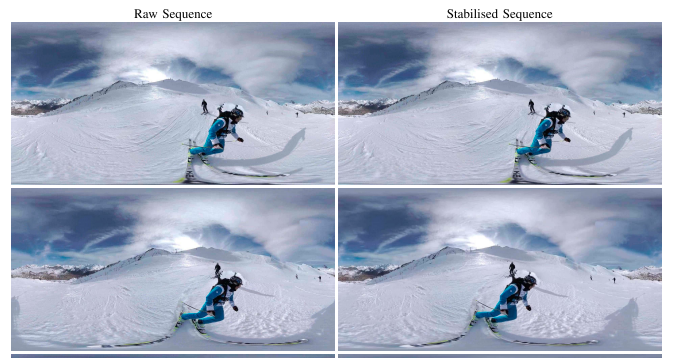
\includegraphics[width=\textwidth]{figures/spherical_video.png}

\section{Variational Auto encoders}

Notations :
\begin{align*}
    z\in\RR^M &: \textrm{latent variables} \\
    x &: \textmd{a vector of $D$ observed variables} \\
    p_\phi(x, z) &: \textrm{a parameterized model of the joint distribution}\\
    q(z) &: \textrm{approximate posterior distribution} \\
    q_\psi(z|x;\theta) &: \textrm{parameterized by a NN that}\\ 
    &\textrm{outputs a probability distribution of $z$ for each data points}
\end{align*}

We want to maximize the log-likelihook of the data by maximizing the Evidence Lower Bound (ELBO).

$$
\mathcal{L}(\phi, \psi) = \EE_{q_{\psi}(z|x; \theta)}[log p_{\phi}(x|z)] - KL(q_{\psi}(z|x;\theta) || p(z))
$$
The first term is the reconstruction loss and the second term is the KL divergence between the approximate posterior and the prior $p(z)$ which is usually $\mathcal{N}(0, 1)$.
Both the prior $p(z)$ and the posterior are defined as normal distributions.

Limitation of gaussian distribution :
\begin{itemize}
    \item Low dimensions : origin gravity
    \item \textcolor{blue}{High dimensions : soap bubble effect}
        \textbf{The standard Gaussian distribution in high dimensions tends to resemble a uniform distribution on the surface of a hypersphere, with the vast majority of its mass concentrated on the hyperspherical shell.}
\end{itemize}

\section{Replacing Gaussian with Von-Mises Fisher}

Analogous to the Gaussian distribution, the vMF is parameterized by $\mu\in\RR^m$ , the mean direction, and $\kappa\in\RR^+$, the concentration parameter around $mu$. For $\kappa=0$, the vMF distribution represents a Uniform distribution on the hypersphere.
For a random unit vector $z\in\RR^m$, ($z\in\mathcal{S}^{m-1}$), the vMF distribution is defined as :
\begin{align*}
    q(z|\mu, \kappa) &= C_m(\kappa) exp(\kappa \mu^T z) \\
    C_m(\kappa) &= \frac{\kappa^{m/2-1}}{(2\pi)^{m/2}I_{m/2-1}(\kappa)} \\
\end{align*}
where $||\mu||^2 =1$, and $I_v$ denotes the modified Bessel function of the first kind of order $v$.
Using the vMF distribution as an approximate posterior, we are able to place a uniform prior on the latent space.
The KL divergence to optimize writes :
\begin{align*}
    KL(q_\psi(z|x; \theta) ||p(z)) &= KL(vMF(\mu, \kappa) || U(S^{m-1})) \\
    &= \kappa\frac{I_{m/2}(k)}{I_{m/2-1}(k)} + log C_m(\kappa) - log\left(\frac{2\pi^{m/2}}{\Gamma(m/2)}\right)^{-1}\\
\end{align*}
Since the KL term does not depend on $\mu$, this is only optimized in the reconstruction term. 
The above expression cannot be handled by automatic differentiation packages because of the modified Bessel function. Thus, we derive the gradient of the KL divergence with respect to $\kappa$. \\ 
\begin{itemize}
    \item \textbf{To sample from vMF} using the procedure of Ulrich \\
        sampling $q(z|e_1, \kappa)$  with $e_1 = (1, 0, \dots, 0)$ using \blue{acceptance-rejection sampling} \\ 
        apply an orthogonal transformation $U$ so that the transformed sampled is distributed according to $q(z|\mu, \kappa)$ \\
        The Householder reflection simply finds an orthonormal transformation $U(\mu)$ that maps vector $e_1$ to $\mu$. \\
        apply $U$ to $z'$ obtained from $w$ and another sample $v$ from a uniform distribution
        \textbf{The sampling technique does not suffer from the curse of dimensionality as we first sample from a univariate distribution}
        
    \item \textbf{Extend the reparametrization trick to vMF}\\ 
    Lemma 2 shows that the distribution can be reparameterized
    \item In high dimension, the surface area collapse to zero (\textit{vanishing surface problem}) $\rightarrow$ unstable behavior of this model in high dimensions
\end{itemize}

\textbf{variational inference} : optimization method that aims at estimating probability distributions with a simpler one \\

\red{acceptance-rejection scheme} : ???  \\ 

\red{Householder reflection} : ??? \\ 

\red{Reparameterization trick} :
How to used backpropagation through the sampling node ? \\
Reparameterization trick enables backpropagation through the sampling node by introducing a deterministic variable (named accepted variable?) $\epsilon$ and a differentiable function $g$ 
such that a sample $z\sim q_\psi(z|x; \theta)$ is expressed as $z=g(\epsilon, \theta, x)$. Indeed, after sampling $epsilon$ during forward pass, it is fixed.
\begin{figure}[!h]
    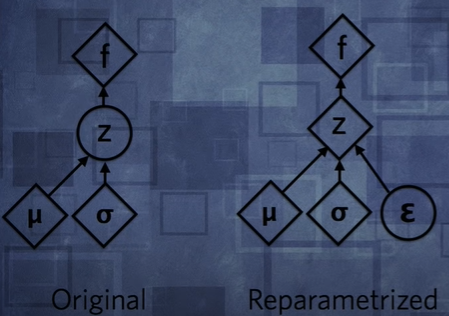
\includegraphics[scale=0.4]{figures/reparametrization.png}
    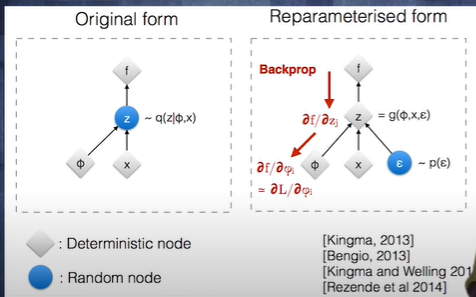
\includegraphics[scale=0.4]{figures/reparam_backprop.png}
\end{figure}

\section{Experiments}

\begin{itemize}
    \item they show that $\mathcal{S}$-VAE outperform $\mathcal{N}$-VAE in recovering a hyperspherical latent structure \\ 
        to investigate theoretical properties of $\mathcal{S}$-VAE \\ 
        \begin{enumerate}
            \item generate samples from three vMFs on the circles, mapped in higher dimension 
            \item train an auto-encoder a $\n$-VAE, a $\Ss$-VAE and a disentangled $\n$-VAE
        \end{enumerate}
    \item thorough comparision with $\mathcal{N}$-VAEs on the MNIST dataset throught an unsupervised and semi-supervised learning task \\
            $\mathcal{S}$-VAE create a better separable latent representation to enhance classification
            (compare on a dataset that does not have a clear hyperspherical latent structure)
            \begin{enumerate}
                \item reconstruction task using MNIST : 
                \item compute ELBO, KL, negative reconstruction error, and marginal log-likelihood (LL) on test data
            \end{enumerate}
                
    \item $\mathcal{S}$-VAEs improve link prediction performance for three citation network datasets in combination with a \textit{Variational Graph Auto-encoder} (VGAE) \\
            data with a non-Euclidean latent representation of low dimensionality 
\end{itemize}


link prediction : ? \\ 
citation network dataset : ?


\section{Conclusion}

\section{My feedbacks / comments / critics}

Code freely available on: https://github.com/ nicola-decao/s-vae

\red{From first meeting held on 2023-11-08} : the project will consist in three important parts :
\begin{itemize}
    \item introduction
    \item present variational auto-encoder (from the paper on \textit{Tutorial on VAE} )
    \item present methods involved in the replacement of gaussians with vMF distributions (sampling and reparametrization trick)
    \item reproduce one experiment from the article, preferably the third one about link prediction on graph : \textit{it is reproduceable with our limited means ?} 
    \item conclusion
\end{itemize}

Possible problems : what criticism related to the course can we make ? 

\end{document}